% !TeX spellcheck = en_US
\documentclass[letterpaper,12pt,twoside]{report}
\usepackage{fancyhdr}
\usepackage{fullpage}
\usepackage{tikz}
\usepackage{amsmath}
\usepackage{textcomp}

\begin{document}
	\pagestyle{fancy}
	\fancyhf{}
	\fancyhead[L]{Day 26}
	\fancyhead[R]{\textit{The Calendar Project}}
	\fancyfoot[L]{Citations Involved: ???}
	
	% Problem
	\paragraph{Problem}
	\begin{quote}
		\textsf{In equilateral triangles $ABC$ and
			$ADE$, $AB=3$  in and $BD = \dfrac{AB}{3}$  in. Find
			the area of the shaded triangle $CDF$.}
	\end{quote}
	
	% Graphics
	\begin{center}
		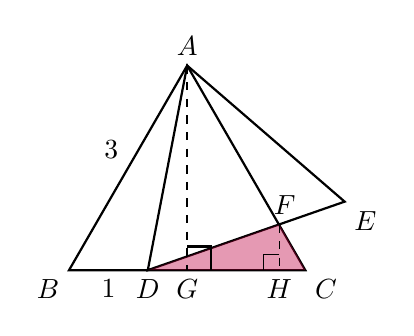
\begin{tikzpicture}
		\draw[thick] (0,0) -- (3,0) -- (1.5,2.598) -- cycle;
		\draw[thick] (1,0) -- (3.5,0.87) -- (1.5,2.598) -- cycle;
		
		\node[above] at (1.5,2.598) {$A$};
		\node[below left] at (0,0) {$B$};
		\node[below right] at (3,0) {$C$};
		\node[below] at (1,0) {$D$};
		\node[below right] at (3.5,0.87) {$E$};
		\node[above] at (2.74,0.58) {$F$};
		
		\draw[fill=purple,opacity=0.4] (3,0) -- (1,0) -- (2.67,0.58);
		
		\node[below] at (0.5,0) {1};
		\node[above left] at (0.75,1.3) {3};
		\node[below] at (1.5,0) {$G$};
		\draw[dashed, thick] (1.5,2.598) -- (1.5,0);
		\draw[thick] (1.5,0.3) -- (1.8,0.3) -- (1.8,0);
		
		\draw[dashed] (2.67,0.58) -- (2.67,0);
		\node[below] at (2.67,0) {$H$};
		\draw (2.67,0.2) -- (2.47,0.2) -- (2.47,0);
		\end{tikzpicture}
	\end{center}
	
	% Reasoning
	\textit{Although approximations are included, no premature rounding is done except to fit the capacity of a floating-point number in Python.}
	\paragraph{Reasoning}
	\begin{quotation}
		
		Given that $AB=3$ and $BD=\frac{AB}{3}$, $BD=\frac{3}{3}=1$, which is denoted above. Draw $\overline{AG}$ from $A$ such that $\overline{AG} \bot \overline{BC}$; this is $\triangle ABC$'s altitude by definition. Given that $\triangle ABC$ and $\triangle ADE$ are equilateral triangles, their sides are congruent: $\overline{AB}\cong\overline{BC}\cong\overline{CA}$ and $\overline{AD}\cong\overline{DE}\cong\overline{EA}$; thus $AB=BC=CA$ and $AD=DE=EA$ by definition. $A$ is on the perpendicular bisector of $\overline{BC}$ by the Converse of the Perpendicular Bisector Theorem; therefore $\overline{AG}$ bisects $\overline{BC}$. By the definition of segment bisection, $\overline{BG}\cong\overline{GC}$ and $BG=GC$. Since $\overline{BC}$ is a side of $\triangle ABC$, $BC=3$; $BG+GC=BC$ by the SAP; $BG+BG=BC$ by substitution, $2BG=BC$ by the distributive property, and $BG=\frac{3}{2}=1.5$. $BD+DG=BG$ by the SAP; with $BD=1$, $1+DG=1.5$ and $DG=1.5-1=0.5$ after subtracting both sides by 1. Since an equilateral triangle is also an equiangular triangle, $\text{m}\angle ABC=\text{m}\angle BCA=\text{m}\angle CAB=\text{m}\angle ADE=\text{m}\angle DEA=\text{m}\angle EAD=60$\textdegree. Since $\overline{AG}\bot\overline{BC}$, $\angle AGB$ and $\angle AGC$ are right angles. With one right angle ($\angle AGB$), $\triangle ABG$ is a right triangle, which makes it eligible for the Pythagorean Theorem (!): $a^2+b^2=c^2 \Rightarrow 1.5^2+AG^2=3^2 \Rightarrow 2.25+AG^2=9$; thus $AG^2=9-2.25=6.75$ and $AG=\sqrt{6.75}\approx 2.598$. In right triangle $ADG$, $\text{m}\angle ADG = \tan^{-1} \frac{AG}{DG}=\tan^{-1} \frac{\sqrt{6.75}}{0.5}\approx 79.1$\textdegree. By the Angle Addition Postulate, $\text{m}\angle CDF+\text{m}\angle FDA=\text{m}\angle CDA \Rightarrow \text{m}\angle CDF+60\approx 79.1$\textdegree. Subtracting 60 from both sides yields $\text{m}\angle CDF\approx 79.1-60=19.1$\textdegree. According to the Triangle Sum Theorem, $\text{m}\angle CDF+\text{m}\angle DFC+\text{m}\angle DCF=180$\textdegree $\Rightarrow (\approx 19.1)+\text{m}\angle DFC+60$\textdegree$=180$\textdegree $\Rightarrow \text{m}\angle DFC=180-60-(\approx 19.1)\approx 100.9$\textdegree. By the SAP, $BD+DC=BC \Rightarrow 1+DC=3 \Rightarrow DC=3-1=2$. By the Law of Sines, $\frac{\sin \angle DFC}{DC}=\frac{\sin \angle DCF}{DF} \Rightarrow \frac{\sin (\approx 100.9)\text{\textdegree}}{2}=\frac{\sin 60\text{\textdegree}}{DF} \Rightarrow \frac{\approx 0.98198}{2}=\frac{\sin 60\text{\textdegree}}{DF}$; by the Cross Product Property, $DF(\approx 0.98198)=2 \sin 60\text{\textdegree} \Rightarrow DF=\frac{2 \sin 60\text{\textdegree}}{\approx 0.98198}\approx 1.763834$. Draw $FH$ from $F$ perpendicular to $\overline{DC}$; this serves as the altitude of $\triangle CDF$ by definition. Because $\overline{FH}$ is perpendicular to $\overline{DC}$, $\angle DHF$ is a right angle and $\triangle DHF$ is a right triangle. $\sin \angle CDF=\frac{FH}{DF}=\frac{FH}{\approx 1.763834}\approx 0.3273 \Rightarrow FH\approx 0.3273 \cdot 1.763734\approx 0.57735$. The triangle area formula is $\frac{1}{2}bh$ where $b$ is the length of its base and $h$ is the length of its height; its application upon $\triangle CDF$ yields $\frac{1}{2}\cdot 2\cdot (\approx 0.57735)\approx \boxed{0.57735 \text{  in}^2}$.
		
		\end{quotation}
	
	\paragraph{External References}
	
	\begin{enumerate}
		\item Textbook Ch. 5, Pg. 300: Converse of the Perpendicular Bisector Theorem
		\item Textbook Ch. 5, Pg. 316: Definition of Triangle Altitude
		\item Textbook Ch. 4, Pg. 223: Triangle Sum Theorem
		\item Textbook Ch. 4, Pg. 224: Corollary (number redacted)
		\item Textbook Ch. 8, Pg. 552: The Law of Sines
	\end{enumerate}
	
\end{document}